\documentclass[12pt, letterpaper, twoside]{article}

\usepackage{geometry}
\usepackage{graphicx}
\usepackage{amsmath, amsfonts, amssymb, bbm}
%\usepackage{lipsum}
\usepackage{fancyhdr}
%\usepackage{layout}
\usepackage{lettrine}

%%%%%%%%%%%%%%%%%%%%%%%% 
% FONT SELECTION  
%%%%%%%%%%%%%%%%%%%%%%%% 

\usepackage[light,math]{iwona}
\usepackage[T1]{fontenc}

%%%%%%%%%%%%%%%%%%%%%%%% 
% PAGE LAYOUT
%%%%%%%%%%%%%%%%%%%%%%%%

% Paper Width 614pt
% Text fill symemetric 604pt
% Paper Height 794pt

\setlength{\voffset}{-0.5in}
\setlength{\hoffset}{-1in}
\setlength{\oddsidemargin}{65pt}
\setlength{\evensidemargin}{45pt}
\setlength{\topmargin}{0in}
\setlength{\headheight}{15pt}
\setlength{\headsep}{20pt}
\setlength{\marginparwidth}{0in}
\setlength{\marginparsep}{0in}
\setlength{\textheight}{635pt}
\setlength{\textwidth}{494pt}
\setlength{\footskip}{50pt}

%%%%%%%%%%%%%%%%%%%%%%%%
% MATH OPERATORS AND 
% CUSTOM ENVIRONMENTS
%%%%%%%%%%%%%%%%%%%%%%%%
\DeclareMathOperator{\Tr}{Tr}
\DeclareMathOperator*{\Cov}{Cov}
\DeclareMathOperator{\cov}{Cov} 
  
\newcounter{observ}
\newenvironment{observ}{\refstepcounter{observ}
   \textit{\textbf{Observation \theobserv:}} \rmfamily}
     
\newenvironment{proof}{\textit{Proof:} \rmfamily}{\hfill$\square$}

\newcommand{\ket}[1]{\ensuremath{\vert #1 \rangle}}
\newcommand{\bra}[1]{\ensuremath{\langle #1 \vert}} 
\newcommand{\braket}[2]{\ensuremath{\langle #1 \vert #2 \rangle}} 
\newcommand{\braOket}[3]{\ensuremath{\langle #1 \vert #2 \vert #3 \rangle}}
\newcommand{\ketbra}[2]{\ensuremath{\vert #1 \rangle \! \langle #2 \vert}}
\newcommand{\meanO}[1]{\ensuremath{\langle #1 \rangle}}
\newcommand{\ver}[2]{\ensuremath{\genfrac{}{}{0pt}{}{#1}{#2}}}
\newcommand{\tr}[1]{\ensuremath{\Tr \lcua #1\rcua}}
\newcommand{\trsub}[2]{\ensuremath{\Tr_{#1} \lcua #2 \rcua }}
\newcommand{\bsym}[1]{\ensuremath{\boldsymbol{#1}}}

\def\be{\begin{equation}}
\def\ee{\end{equation}}
\def\bea{\begin{eqnarray}}
\def\eea{\end{eqnarray}}
\def\bse{\begin{subequations}} 
\def\ese{\end{subequations}}
\def\mtxid{\mathbbm{1}}
\def\lpar{\left(} 
\def\rpar{\right)}
\def\lcua{\left[}
\def\rcua{\right]}
\def\lcor{\left\{}
\def\rcor{\right\}}
\def\lang{\left\langle}
\def\rang{\right\rangle}
\def\l{\left} 
\def\r{\right}
\def\nnnl{\nonumber\\}
\def\nnnlq{\nonumber\\ && \quad}
\def\nnnlqq{\nonumber\\ && \qquad}
\def\nnnlqqq{\nonumber\\ && \quad\qquad}
\def\ie{, \textit{i.e.}, }

%%%%%%%%%%%%%%%%%%%%%%%%
% DOCUMENT
%%%%%%%%%%%%%%%%%%%%%%%%
\begin{document}

\pagestyle{fancy}
\renewcommand{\sectionmark}[1]{\markboth{}{\MakeUppercase{\emph{#1}}}}
\renewcommand{\subsectionmark}[1]{\markboth{\emph{#1}}{}}
\renewcommand{\headrulewidth}{0pt}
\fancyhead{}
\fancyfoot{}

%%%%%%%%%%%%%%%%%%%%%%%%
% TITLE PAGE
%%%%%%%%%%%%%%%%%%%%%%%%

%!TEX root = main.tex 

\thiswatermark{\centering
\put(0,-110){
\includegraphics[height=2.5cm]{img/0-Ztf.png}} 
\put(430,-100){
\includegraphics[height=2cm]{img/0-Ehu.png}}
} 

\begin{center}

\vspace*{20pt}
\textsc{\LARGE University of the Basque Country}

\vspace{20pt}
\textsc{\Large PhD Thesis}

\vspace{50pt} 
\hrule 

\vspace{16pt}
{\huge \bfseries Lower bounds on quantum metrological precisions}
\vspace{16pt}

\hrule
\vspace{40pt}

\begin{minipage}{0.4\textwidth}
\begin{flushleft} \large
\emph{Author:}


M. Sc. Iagoba \textsc{Apellaniz}
\end{flushleft}
\end{minipage}
\begin{minipage}{0.4\textwidth}
\begin{flushright} \large
\emph{Director:}

Prof. G\'eza \textsc{T\'oth} %TODO: Check Geza's name
\end{flushright}
\end{minipage}

\vspace{40pt}
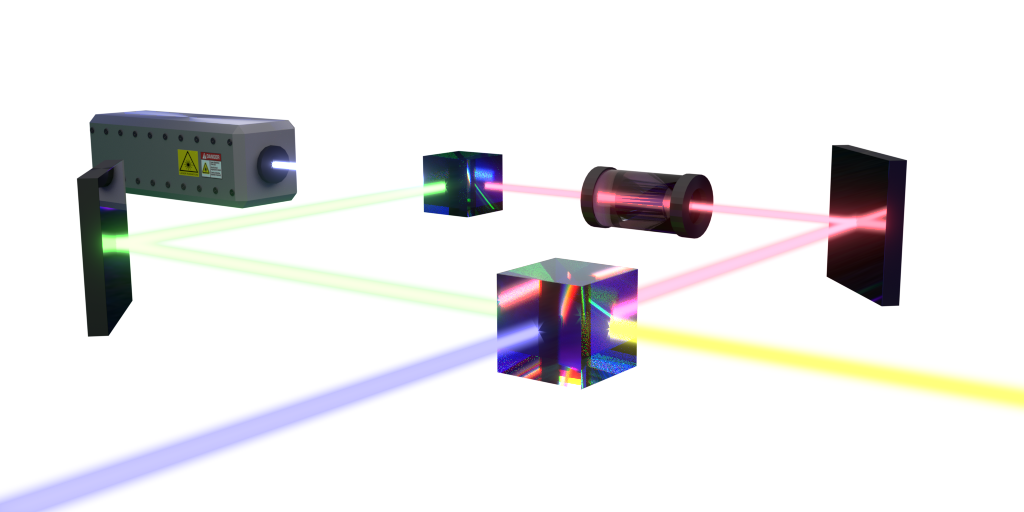
\includegraphics[width=0.8\hsize]{img/cover3Dpicture.png}
\vfill

% Bottom of the page
{\large \today}

\end{center}

\cleardoublepage

%%%%%%%%%%%%%%%%%%%%%%%%
% EDITION TIPS
%%%%%%%%%%%%%%%%%%%%%%%%

\cleardoublepage

This document was generated with the 2013 distribution of \LaTeX. 

%%%%%%%%%%%%%%%%%%%%%%%%
% PROLOGE
%%%%%%%%%%%%%%%%%%%%%%%%

\cleardoublepage
\setcounter{page}{1}
\pagenumbering{roman}

\fancyfoot[LE,RO]{\thepage}

\vspace*{100pt}
\section*{Prologue}
\vspace{50pt}

Here is the prologue.

%%%%%%%%%%%%%%%%%%%%%%%%
% TABLE OF CONTENTS
%%%%%%%%%%%%%%%%%%%%%%%%

\cleardoublepage

\vspace*{100pt}
\tableofcontents

%%%%%%%%%%%%%%%%%%%%%%%%
% THESIS
%%%%%%%%%%%%%%%%%%%%%%%%

\cleardoublepage
\setcounter{page}{1}
\pagenumbering{arabic}
\fancyfoot{}

%!TEX root = main.tex 

\thiswatermark{\centering
\put(0,-110){
\includegraphics[height=2.5cm]{img/0-Ztf.png}} 
\put(430,-100){
\includegraphics[height=2cm]{img/0-Ehu.png}}
} 

\begin{center}

\vspace*{20pt}
\textsc{\LARGE University of the Basque Country}

\vspace{20pt}
\textsc{\Large PhD Thesis}

\vspace{50pt} 
\hrule 

\vspace{16pt}
{\huge \bfseries Lower bounds on quantum metrological precisions}
\vspace{16pt}

\hrule
\vspace{40pt}

\begin{minipage}{0.4\textwidth}
\begin{flushleft} \large
\emph{Author:}


M. Sc. Iagoba \textsc{Apellaniz}
\end{flushleft}
\end{minipage}
\begin{minipage}{0.4\textwidth}
\begin{flushright} \large
\emph{Director:}

Prof. G\'eza \textsc{T\'oth} %TODO: Check Geza's name
\end{flushright}
\end{minipage}

\vspace{40pt}
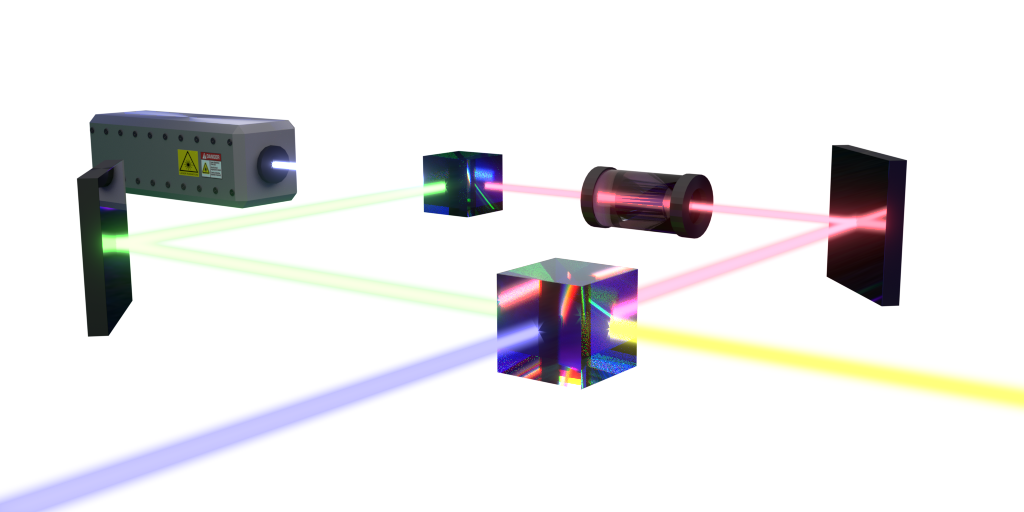
\includegraphics[width=0.8\hsize]{img/cover3Dpicture.png}
\vfill

% Bottom of the page
{\large \today}

\end{center}

\cleardoublepage

\cleardoublepage
\vspace*{100pt}
\begin{center}
\emph{To my parents and my family}
\end{center}

\cleardoublepage

\renewcommand{\headrulewidth}{1pt}
\fancyfoot[LE,RO]{\thepage}
\fancyhead[LE]{\rightmark}
\fancyhead[RO]{\leftmark} 
 
\vspace*{100pt}
\section{Introduction}
\vspace{50pt}

\lettrine[lines=2, findent=3pt,nindent=0pt]{I}{n} recent years many work and
implementations of quantum metrology arise to the public domain.
The interest of this field is increasing day by day.

\cleardoublepage
\vspace*{100pt}
\section{Accuracy Bounds for Gradient Estimation with Atom Ensembles}
\vspace{50pt}

\subsection{States insensitive to the homogeneous field as prove states}

\subsubsection{Single-Cloud ensemble of Atoms}

\subsubsection{Twin-Cloud ensemble}

\subsection{Usefulness of states sensitive to the homogeneous field}



\end{document}
